%\title{Project Report}
%
%%% Preamble
\documentclass[paper=a4, fontsize=11pt]{scrartcl}
\usepackage[T1]{fontenc}
\usepackage{fourier}

\usepackage[english]{babel}															% English language/hyphenation
\usepackage[protrusion=true,expansion=true]{microtype}
\usepackage{amsmath,amsfonts,amsthm} % Math packages
\usepackage[pdftex]{graphicx}
\usepackage{url}
\usepackage{listings}
\usepackage[final]{pdfpages}
\usepackage[section]{placeins}

%%% Custom sectioning
\usepackage{sectsty}
\allsectionsfont{\centering \normalfont\scshape}


%%% Custom headers/footers (fancyhdr package)
\usepackage{fancyhdr}
\pagestyle{fancyplain}
\fancyhead{}											% No page header
\fancyfoot[L]{}											% Empty
\fancyfoot[C]{}											% Empty
\fancyfoot[R]{\thepage}									% Pagenumbering
\renewcommand{\headrulewidth}{0pt}			% Remove header underlines
\renewcommand{\footrulewidth}{0pt}				% Remove footer underlines
\setlength{\headheight}{13.6pt}


%%% Equation and float numbering
\numberwithin{equation}{section}		% Equationnumbering: section.eq#
\numberwithin{figure}{section}			% Figurenumbering: section.fig#
\numberwithin{table}{section}				% Tablenumbering: section.tab#


%%% Maketitle metadata
\newcommand{\horrule}[1]{\rule{\linewidth}{#1}} 	% Horizontal rule

\title{
		%\vspace{-1in}
		\usefont{OT1}{bch}{b}{n}
		\normalfont \normalsize \textsc{University of Michigan} \\ [25pt]
		\horrule{0.5pt} \\[0.4cm]
		\huge AERO 584, Final Exam \\
		\horrule{2pt} \\[0.5cm]
}
\author{
		\normalfont 								\normalsize
         Huckleberry Febbo\\[-3pt]		\normalsize
        \today
}
\date{}

%%%%%%%%%%%%%%%%%%%%%%%%%%%%%%%%%%%%%%%%%%%%%%%%%%%%%%%%%%%%%%%%%%%%%
%%%%%%%%%%%%%%%%%%%%%%%%%%%%%%%%PACKAGES%%%%%%%%%%%%%%%%%%%%%%%%%%%%%%%%

% *** MATH ***
\usepackage{amsmath}
\usepackage{cases}
\usepackage{mathrsfs}
\usepackage{amssymb}
\DeclareMathAlphabet\mathbfcal{OMS}{cmsy}{b}{n}


% *** GRAPHICS ***
\usepackage[]{graphicx}
\usepackage{epstopdf}
\usepackage{svg}
\setsvg{inkscape=inkscape -z -D,svgpath=figs/}

\usepackage{lineno,hyperref}
\modulolinenumbers[5]


\bibliographystyle{elsarticle-num}
%%%%%%%%%%%%%%%%%%%%%%%

\begin{document}
\maketitle

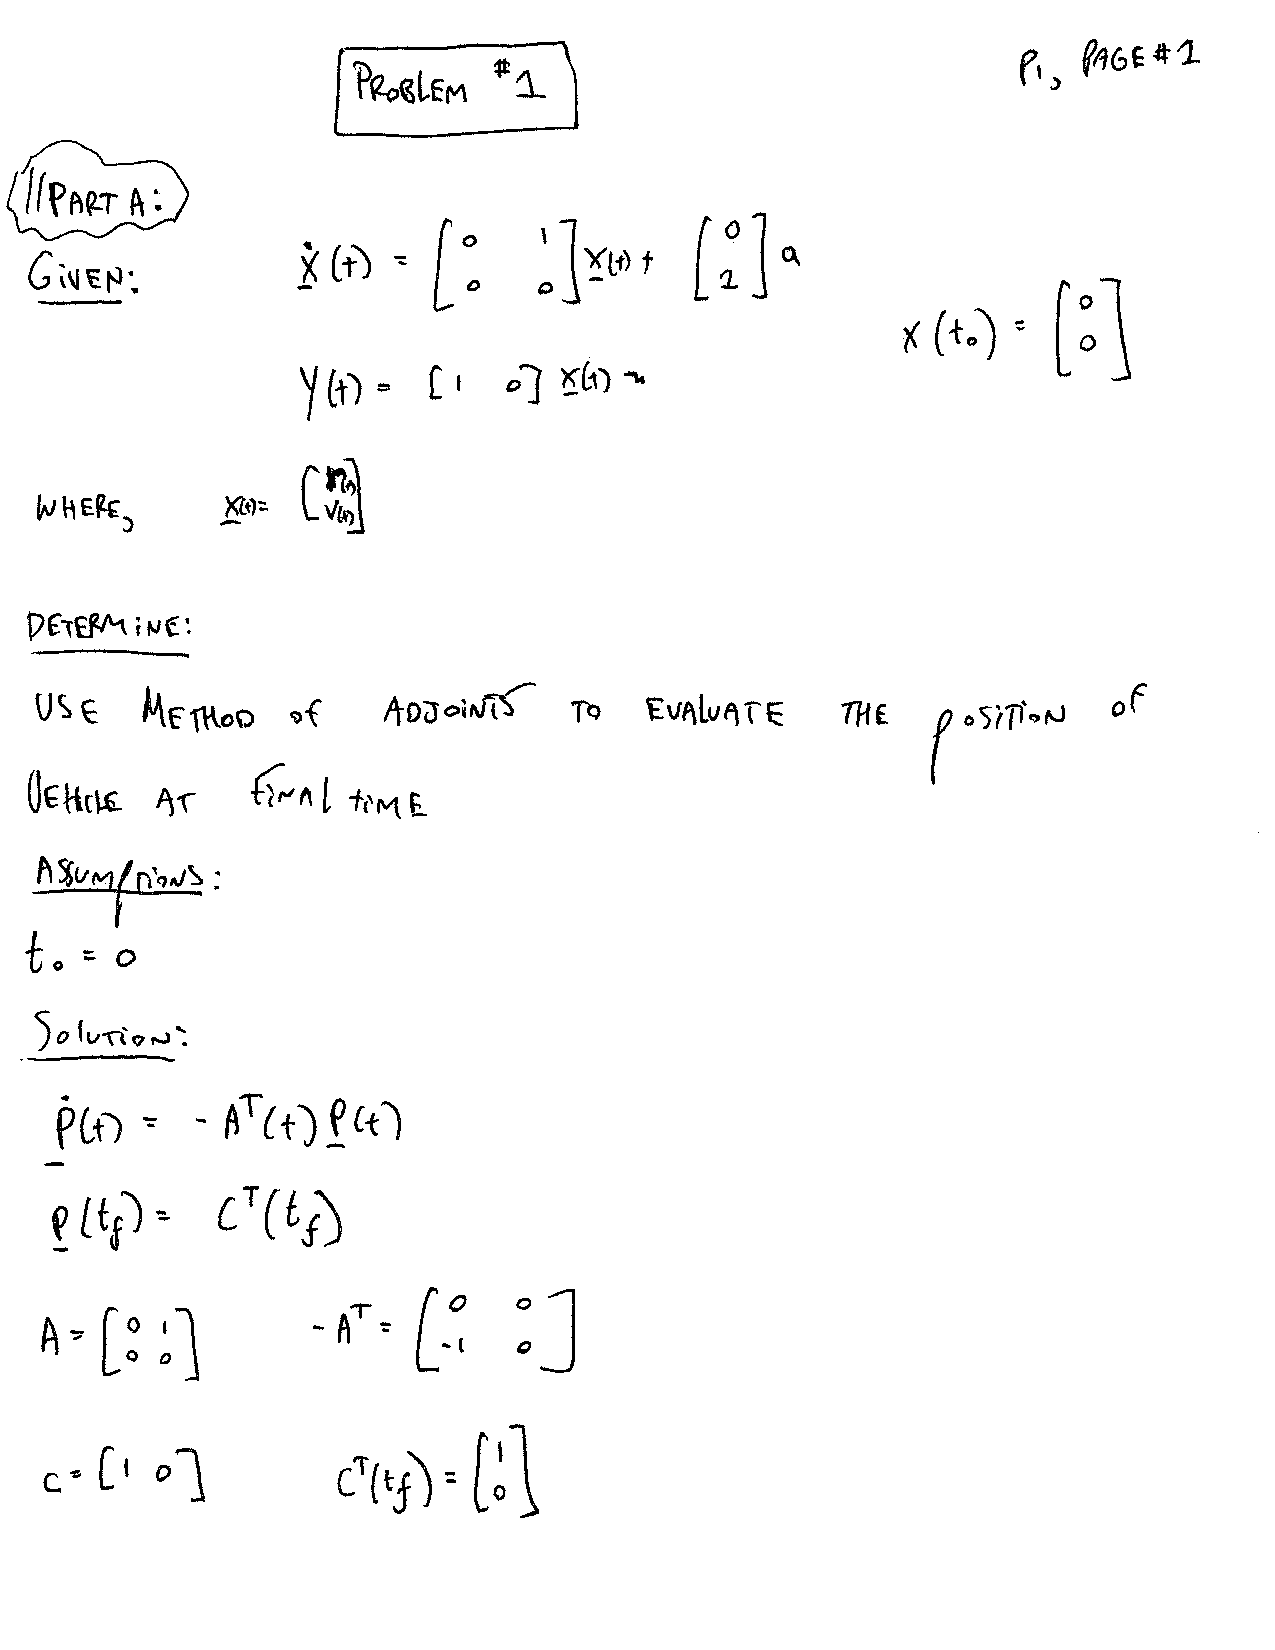
\includepdf[pages=-]{a.pdf}


\section*{Problem 4, part a}
First, for a sanity check, in Fig. \ref{fig:q1}-\ref{fig:q2}, the position of the MAV using the Vicon data is plotted against the position of the MAV calculated using the data given (assumed) for the GV, the quaternion data transformed to a rotation matrix and the given data for eB. It can be seen that there is an offset for the two trajectories in the $x$ direction.
\footnote{For posterity, the code that produced the results for Problem 4 is included in the appendix}
\begin{figure}[!htb]
	\centering
    \includesvg[width=0.9\textwidth]{p4a}
	\caption{  \label{fig:q1}}
\end{figure}

\begin{figure}[!htb]
	\centering
    \includesvg[width=0.9\textwidth]{p4b}
	\caption{  \label{fig:q2}}
\end{figure}

Next, after formulating a Kalman Filter for the closed loop system, the resulting trajectories for eB are compared to the given data for eB in Fig. \ref{fig:g3}. It can be seen that the trajectory determined using the Kalman Filter is offset from the data that was given for eB for both the $x$ and the $y$, but the $z$ matches fairly closely. 

\begin{figure}[!htb]
	\centering
    \includesvg[width=0.9\textwidth]{p4c}
	\caption{  \label{fig:q3}}
\end{figure}

Finally, the trajectory for $xW$ is plotted for both the Vicon system as well as the trajectory transformed from the $eB$ trajectory determined using the Kalman Filter (shown in Fig. \ref{fig:g3}) to the $W$ frame is shown in Fig. \ref{fig:q4}. Again there is an offset for both the $x$ and the $y$, but the $z$ matches fairly closely.

\begin{figure}[!htb]
	\centering
    \includesvg[width=0.9\textwidth]{p4e}
	\caption{  \label{fig:q4}}
\end{figure}



\section*{Problem 4, part b}

For this set of results, the covariance matrix for the noise is increased as mentioned in the problem statement. All of the same results where collected and are shown in Figs. \ref{fig:q4}-\ref{fig:q5}. Again, we see an offset for both the $x$ and the $y$, but now the $z$ has an offset as well.  When compared to the results in Part a, there is a degradation in the estimate that the Kalman Filter is performing, this is especially evident when considering that there is now an offsest in $z$ as well and that the offsets are larger for $x$ and $y$ as well.

\begin{figure}[!htb]
	\centering
    \includesvg[width=0.9\textwidth]{p4cB}
	\caption{  \label{fig:q5}}
\end{figure}

\begin{figure}[!htb]
	\centering
    \includesvg[width=0.9\textwidth]{p4eB}
	\caption{  \label{fig:q6}}
\end{figure}

\section*{Problem 5, part a}
In Fig. \ref{fig:f1} it can be seen that Iron Man is able to hit the target.
\begin{figure}[!htb]
	\centering
	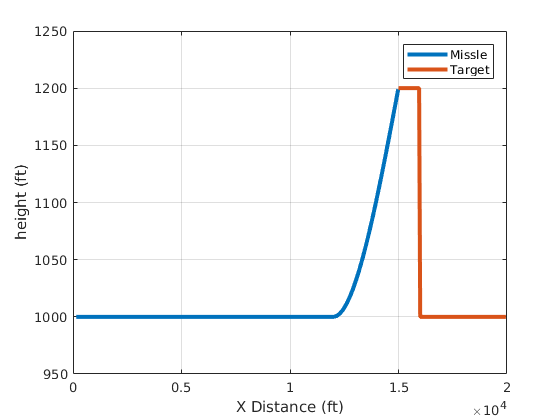
\includegraphics[width=0.7\textwidth]{fivea}
	\caption{ Position tracjectories of Iron Man and his target, when Time-to-Go $= 1s$ \label{fig:f1}}
\end{figure}

\section*{Problem 5, part b}
In Fig. \ref{fig:f2} it can be seen that the acceleration is very large for Iron Man to perform the maneuver in Fig. \ref{fig:f1}.
\begin{figure}[!htb]
	\centering
	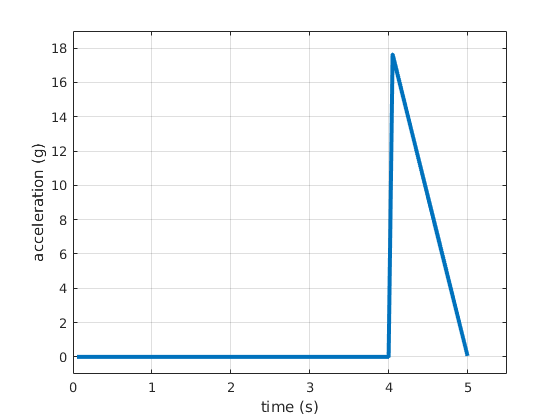
\includegraphics[width=0.7\textwidth]{fiveb}
	\caption{ Acceleration required by Iron Man so the he catches the destructive square\label{fig:f2}}
\end{figure}

\section*{Problem 5, part c}
It can be seen in Fig. \ref{fig:f4} that as the Time-To-Go is increased the acceleration required by Iron Man to hit the target is decreased. This can also be seen in Fig. \ref{fig:f5}, where Iron Man is allowed to start moving at the start of the simulation.
\begin{figure}[!htb]
	\centering
	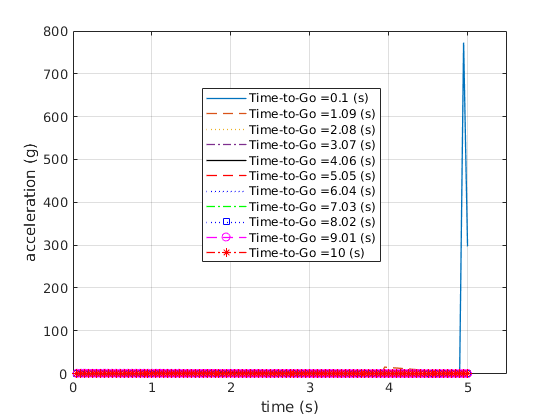
\includegraphics[width=0.7\textwidth]{fivec1}
	\caption{ Acceleration required by Iron Man for various Time-to-Go's form $0.1sec \rightarrow 10sec$\label{fig:f3}}
\end{figure}

\begin{figure}[!htb]
	\centering
	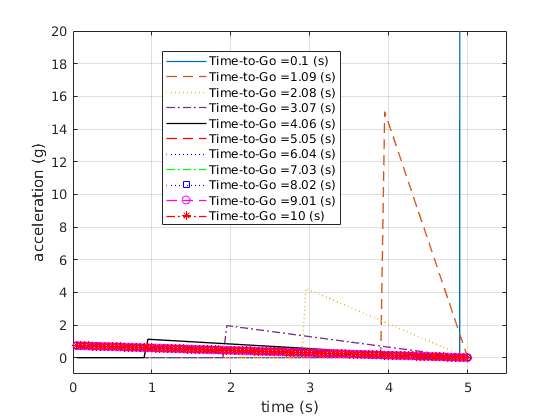
\includegraphics[width=0.7\textwidth]{fivec2}
	\caption{ Zoomed in plot of acceleration required by Iron Man for various Time-to-Go's from $0.1sec \rightarrow 10sec$\label{fig:f4}}
\end{figure}

\begin{figure}[!htb]
	\centering
	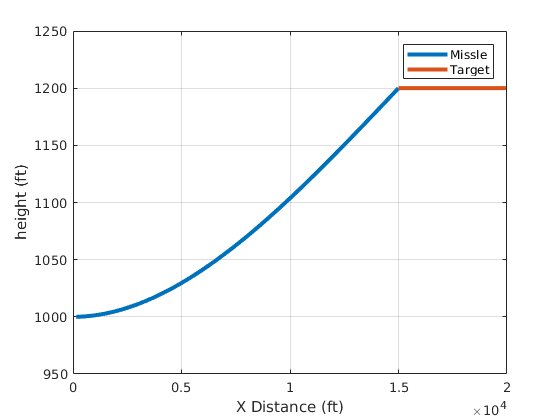
\includegraphics[width=0.7\textwidth]{fivec3}
	\caption{ Just for fun, a look at the position plot when Time-to-go $=10sec$\label{fig:f5}}
\end{figure}

\section*{Problem 5, part a.2}
In Fig. \ref{fig:f6}, when Iron Man cannot instantaneously track the target and there is a first-order dynamics with $T=1$. In this case, it can be seen that Iron Man misses the target. 
\begin{figure}[!htb]
	\centering
	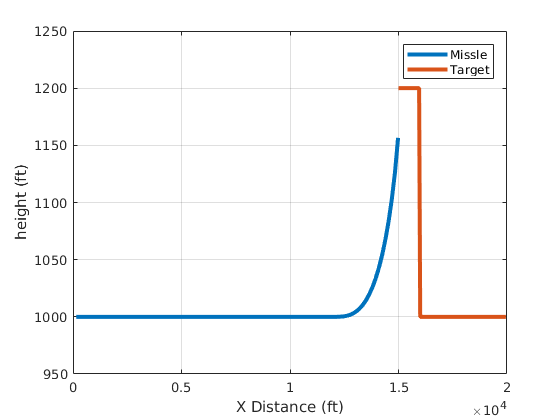
\includegraphics[width=0.7\textwidth]{fivea2}
	\caption{ Position tracjectories of Iron Man and his target, when Time-to-Go $= 1s$ \label{fig:f6}}
\end{figure}

\section*{Problem 5, part b.2}
In Fig. \ref{fig:f7} the miss distance for the Time-to-Go = 1s \footnote{assuming that the Time-To-Go is still $=1 s$, as given in the original problem statement} is shown by the red dot. It can be seen that that the miss distance is $= 38.94 (ft)$. 
\begin{figure}[!htb]
	\centering
	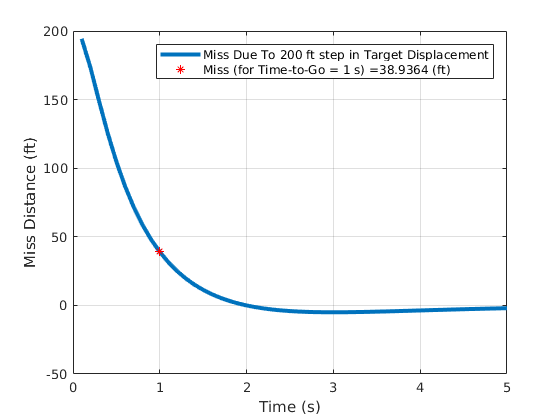
\includegraphics[width=0.7\textwidth]{fiveb2}
	\caption{ Position tracjectories of Iron Man and his target, when Time-to-Go $= 1s$ \label{fig:f7}}
\end{figure}


\section*{Problem 4, julia code}
\begin{lstlisting}
using Plots
pgfplots()
using LaTeXStrings
PGFPlots.pushPGFPlotsPreamble("\\usepackage{amssymb}")
using Interpolations
using OrdinaryDiffEq
using DiffEqBase
using DataFrames

d = readtable("data.csv")

# extract data
t = d[:t]; # seconds
XxV = d[:XxV]
XyV = d[:XyV]
XzV = d[:XzV]
qx = d[:qx]
qy = d[:qy]
qz = d[:qz]
qw = d[:qw]
ZxW = d[:ZxW]
ZyW = d[:ZyW]
ZzW = d[:ZzW]
ExB = d[:ExB]
EyB = d[:EyB]
EzB = d[:EzB]
eta = d[:eta]
E1I = d[:E1I]
E2I = d[:E2I]
E3I = ones(length(E2I))

lambda = abs(EzB)

# misc variables
L = length(t)
l1 = (6,:green,:solid)
l2 = (3,:red,:solid)
l3 = (2.2,:black,:dash)
l4 = (1.5,:blue,:dot)

# rotation matrix, https://en.wikipedia.org/wiki/Conversion_between_quaternions_and_Euler_angles
function ROT(q_x,q_y,q_z,q_w)
   [1 - 2*(q_y^2 + q_z^2)       2*(q_x*q_y - q_w*q_z)     2*(q_w*q_y + q_x*q_z);
    2*(q_x*q_y + q_w*q_z)       1-2*(q_x^2 + q_z^2)       2*(q_z*q_y - q_w*q_x);
    2*(q_x*q_z - q_w*q_y)       2*(q_z*q_y + q_w*q_x)     1-2*(q_y^2 + q_x^2)];
end

# direction cosine matrices, 3-2-1 sequence (psi,theta,phi)
# [x,y,z] = Rz(psi)*Ry(theta)*Rz(phi)[X;Y;Z]
function Rz(psi)
 [cos(psi) -sin(psi) 0;
  sin(psi)  cos(psi) 0;
     0         0     1]
end

function Ry(theta)
 [cos(theta)       0   sin(theta);
      0            1       0;
  -sin(theta)      0     cos(theta)]
end

function Rx(phi)
 [1         0       0;
  0       cos(phi) -sin(phi);
  0       sin(phi)  cos(phi)]
end

##################
# part a)
K_intr = [1030.597415177913           0          361.451236121491;
                  0           1030.358516382353  246.1238464630347;
                  0                   0                1]
C_intr = [1  0  0;
          0 -1  0;
          0  0 -1]

KK = [ 0.5   0     0;
      0    0.6    0;
      0     0   0.07]

rotM = zeros(L,3,3)
eB = zeros(L,3)
eBM = zeros(L,3)
xW = zeros(L,3)

for i in 1:L-1
 # calculate rotation matrix using quaternion data from Vicon system
 rotM[i,:,:] = ROT(qx[i],qy[i],qz[i],qw[i])
 # put eB into a matrix
 eB[i,:] = [ExB[i];EyB[i];EzB[i]]
 # calculate eB from the measured data
 eI = [E1I[i];E2I[i];E3I[i]]
 eBM[i,:] = inv(C_intr)*inv(KK)*lambda[i]*eI
 # estimate xW from vectors
 xW[i,:] = [-ZxW[i];ZyW[i];ZzW[i]] - rotM[i,:,:]*eB[i,:,:]
end
wB = zeros(L,3,3)
for i in 1:L-1
 dt = d[:t][i+1] - d[:t][i]
 wB[i,:,:] = (rotM[i+1,:,:] - rotM[i,:,:])/dt
end
# xW) plots
s1 = "using Vicon"
s2 = "calcualted "

plot(XxV,XyV,XzV,line=l1,label=s1)
plot!(xW[:,1],xW[:,2],xW[:,3],line=l2,label=s2,cbar=false)
savefig(string("figs/p4a",".",:svg));

# position
p1 = plot(t,XxV,line=l1,label=s1)
plot!(t,xW[:,1],line=l2,label=s2)
yaxis!("x (m)")
xaxis!("Time (s)")

p2 = plot(t,XyV,line=l1,label=s1)
plot!(t,xW[:,2],line=l2,label=s2)
yaxis!("y (m)")
xaxis!("Time (s)")

p3 = plot(t,XzV,line=l1,label=s1)
plot!(t,xW[:,3],line=l2,label=s2)
yaxis!("z (m)")
xaxis!("Time (s)")
plot(p1,p2,p3,layout=@layout([a;b;c]),size=[600,600])
savefig(string("figs/p4b",".",:svg));

Rw = zeros(6,6)
Rw[1:3,1:3] = [0.1    0   0;
                0   0.1   0;
                0     0  0.1]
Rv= [2 0 0;
     0 2 0;
     0 0 2]
x_k = zeros(L); x_k[1] = 0;
y_k = zeros(L); y_k[1] = 0;
z_k = zeros(L); z_k[1] = 0;
vx_k = zeros(L); vx_k[1] = 0;
vy_k = zeros(L); vy_k[1] = 0;
vz_k = zeros(L); vz_k[1] = 0;
x = zeros(L,6); x[1,1:6] = [0,0,0,0,0,0];
P = zeros(L,6,6)
for i in 1:L-1
 dt = d[:t][i+1] - d[:t][i]
 A = [1  0  0  dt 0   0;
      0  1  0  0  dt  0;
      0  0  1  0  0  dt;
      0  0  0  1  0   0;
      0  0  0  0  1   0;
      0  0  0  0  0   1]

 B = [1   0  0;
      0   1  0;
      0   0  1;
      0   0  0;
      0   0  0;
      0   0  0]

 C = [1 0  0 dt 0   0;
      0 1  0 0  dt  0;
      0 0  1 0  0  dt]

 # time update (predict)
 u = (-wB[i,:,:] + KK)
 x[i+1,:] = A*x[i,:] + B*[u[1,1];u[2,2];u[3,3]]
 P[i+1,:,:] = A*P[i,:,:]*A' + Rw

 # measurment update
 eI = [E1I[i];E2I[i];E3I[i]]
 y = inv(C_intr)*inv(K_intr)*lambda[i]*eI
 K = P[i+1,:,:]*C'*inv((C*P[i+1,:,:]*C' + Rv))
 x[i+1,:] = x[i+1,:] + K*(y-C*x[i+1,:])
 P[i+1,:,:] = (eye(6) - K*C)*P[i+1,:,:]

 # save results
 x_k[i+1] = x[i+1,1]
 vx_k[i+1] = x[i+1,4]

 y_k[i+1] = x[i+1,2]
 vy_k[i+1] = x[i+1,5]

 z_k[i+1] = x[i+1,3]
 vz_k[i+1] = x[i+1,6]
end

# part a) plot eB
s1 = "given eB"
s2 = "eB using Kalman Filter"

# position
p1 = plot(t,eB[:,1],line=l1,label=s1)
plot!(t,x_k,line=l2,label=s2)
yaxis!("x (m)")
xaxis!("Time (s)")

p2 = plot(t,eB[:,2],line=l1,label=s1)
plot!(t,y_k,line=l2,label=s2)
yaxis!("y (m)")
xaxis!("Time (s)")

p3 = plot(t,eB[:,3],line=l1,label=s1)
plot!(t,z_k,line=l2,label=s2)
yaxis!("z (m)")
xaxis!("Time (s)")
plot(p1,p2,p3,layout=@layout([a;b;c]),size=[600,600])
savefig(string("figs/p4c",".",:svg));

plot(eB[:,1],eB[:,2],eB[:,3],line=l1,label=s1,cbar=false)
plot!(x_k,y_k,z_k,line=l2,label=s2,cbar=false,size=[800,800])
xaxis!("x (m)")
yaxis!("y (m)")
savefig(string("figs/p4d",".",:svg));

# xWK)
xWK = zeros(L,3)
for i in 1:L-1
 # estimate xWK from vectors
 xWK[i,:] = [-ZxW[i];ZyW[i];ZzW[i]] - rotM[i,:,:]*[x_k[i];y_k[i];z_k[i]]
end

s1 = "xW using Vicon"
s2 = "xW using Kalman Filter"

# position
p1 = plot(t,XxV,line=l1,label=s1)
plot!(t,xWK[:,1],line=l2,label=s2)
yaxis!("x (m)")
xaxis!("Time (s)")

p2 = plot(t,XyV,line=l1,label=s1)
plot!(t,xWK[:,2],line=l2,label=s2)
yaxis!("y (m)")
xaxis!("Time (s)")

p3 = plot(t,XzV,line=l1,label=s1)
plot!(t,xWK[:,3],line=l2,label=s2)
yaxis!("z (m)")
xaxis!("Time (s)")
plot(p1,p2,p3,layout=@layout([a;b;c]),size=[600,600])
savefig(string("figs/p4e",".",:svg));

plot(XxV,XyV,XzV,line=l1,label=s1,cbar=false)
plot!(xWK[:,1],xWK[:,2],xWK[:,3],line=l2,label=s2,cbar=false,size=[800,800])
xaxis!("x (m)")
yaxis!("y (m)")
savefig(string("figs/p4f",".",:svg));
\end{lstlisting}
\end{document}
